
\lecture{Assessing Normality}{assessing-normality}
\section{Assessing Normality}

\title{Assessing Normality}
\subtitle{What is the Distribution?}

%\author{Kelly Black}
%\institute{Clarkson University}
\date{22 Feb 2012}

\begin{frame}
  \titlepage
\end{frame}

\begin{frame}
  \frametitle{Outline}
  \tableofcontents[hideothersubsections,sectionstyle=show/hide]
\end{frame}


\iftoggle{clicker}{%
  \subsection{Clicker Quiz}


  \begin{frame}
    \frametitle{Clicker Quiz}

    Determine the first quartile (Q1) for the following data: \\
    \begin{tabular}{llllll}
      17 & 16 & 18 & 18 & 13 & 15 
    \end{tabular}
 
    \vfill

    \begin{tabular}{l@{\hspace{3em}}l@{\hspace{3em}}l}
      A:  15 & B: 16 & C: 16.5
    \end{tabular}

    \vfill
    \vfill
    \vfill

  \end{frame}
}




\subsection{Assessing Normality}

\begin{frame}
  \frametitle{Given Data Is It Normally Distributed?}

  Given a set of data you want to know if it is consistent with some
  distribution. Here we focus on the normal distribution. 

  The Idea - \textbf{If the data is normally distributed then}
  \begin{itemize}
  \item You can calculate a $z$-statistic for each number in the data
    set.
  \item The percentile of each $z$-statistic should be consistent with
    the corresponding percentile within the data.
  \item If you plot the actual $z$-statistic as a function of the
    theoretical $z$-statistic of the data point's percentile it should
    give a straight line.
  \end{itemize}
  
\end{frame}

\begin{frame}
  \frametitle{Normal Probability Plot}

  Given a data set,
  \begin{eqnarray*}
    y_1,~y_2,~y_3,\ldots,y_n,
  \end{eqnarray*}
  we construct a normal probability plot to provide an initial
  estimate how closely the data conforms to a normal distribution.

  \begin{enumerate}
    \only<1>{\item Sort the data from low to high,
      \begin{eqnarray*}
        x_1,~x_2,~x_3,\ldots,x_n, \\
        x_i & \leq & x_{i+1}.
      \end{eqnarray*}}
  \only<1>{\item Calculate the sample mean,
    \begin{eqnarray*}
      \bar{x} & = & \frac{x_1+x_2+\cdots+x_n}{n}.
    \end{eqnarray*}}
  \only<1>{\item Calculate the sample standard deviation,
    \begin{eqnarray*}
      s^2 & = & \frac{(x_1-\bar{x})^2 + \cdots + (x_n-\bar{x})^2}{n-1}, \\
      s & = & \sqrt{s^2}.
    \end{eqnarray*}}
  \only<2>{\item For each data point compute its percentile within the data
    assuming a normal distribution,
    \begin{eqnarray*}
      f_i & = & \frac{i-\frac{3}{8}}{n+\frac{1}{4}}.
    \end{eqnarray*}}
  \only<2>{\item Calculate the $z$-statistic associated with $f_i$ by working
    the standard normal table backwards to get $Z^*_i$.}
  \only<2>{\item Calculate the $z$-statistic associated with $x_i$ using
    \begin{eqnarray*}
      z_i & = & \frac{x_i-\bar{x}}{s}.
    \end{eqnarray*}}
  \only<2>{\item Plot each data pair, $(z_i,Z^*_i)$, on a plot. }
  \end{enumerate}
  
\end{frame}

\begin{frame}
  \frametitle{Example}

  First, nobody does this by hand without begging for mercy before it
  is done. This is something that is done on a computer.

  \begin{columns}

    \column{.4\textwidth}
    Given the data, \\
    \begin{tabular}{llllll}
      17 & 16 & 18 & 18 & 13 & 15
    \end{tabular} \\
    The normal probability plot is shown.

  \column{.5\textwidth}

  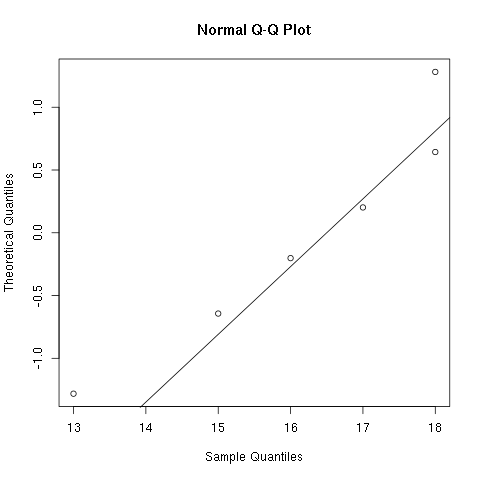
\includegraphics[width=5cm]{img/normalQQEx1}

  \end{columns}
  
  
\end{frame}

\begin{frame}
  \frametitle{Example}


  \begin{columns}

    \column{.4\textwidth}
    Given the data, \\
    \begin{tabular}{llllll}
      9 & 12 & 11 & 8 & 10 & 12
    \end{tabular} \\
    The normal probability plot is shown.

  \column{.5\textwidth}

  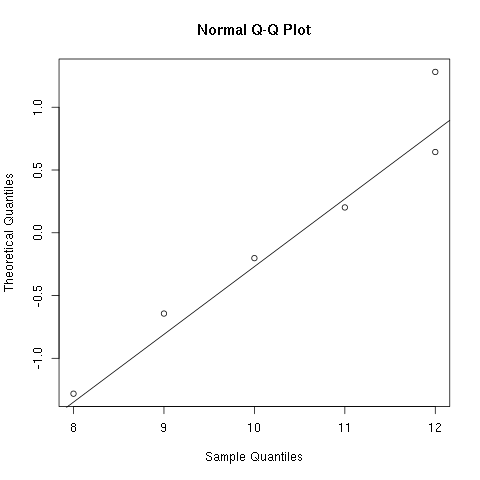
\includegraphics[width=5cm]{img/normalQQEx2}

  \end{columns}
  
  
\end{frame}


%%% Local Variables: 
%%% mode: latex
%%% TeX-master: "IntroStats"
%%% End: 
